%%%%%%%%%%%%%%%%%%%%%%%%%%%%%%↓設定↓%%%%%%%%%%%%%%%%%%%%%%%%%%%%%
%このフォーマットは第26回HISS査読用論文フォーマットです.
%同封の26thHISS.styも作業フォルダにコピーしてお使いください.
\documentclass[a4j,twocolumn,10pt]{jarticle}
\usepackage{26thHISS}
\headsep=0mm
\textheight=24cm
%%%%%%%%%%%%%%%%%%%%%%%%%%%%%%↑設定↑%%%%%%%%%%%%%%%%%%%%%%%%%%%%%
\usepackage[dvipdfmx]{graphicx}
\usepackage[subrefformat=parens]{subcaption}

% \usepackage[ipa]{pxchfon}
% \setminchofont{ipam.ttf}
% \setgothicfont{ipag.ttf}

\title{ 
  セマンティックセグメンテーションを用いた水面領域抽出のための半自動アノテーション手法 \\
  Semi-automatic annotation method for extracting water surface regions using semantic segmentation
}

\author{%
中島慶$^{\dagger}$ 島和之$^{\dagger}$ \\
Kei Nakashima$^{\dagger}$ Kazuyuki Shima$^{\dagger}$ \\
$^{\dagger}$広島市立大学 情報科学研究科\hspace*{1em}
}

\begin{document}
\maketitle
\thispagestyle{empty} %%←消さない%%
\pagestyle{empty} %%←消さない%% 追加 2006.10.13
\baselineskip=4.5mm %%←消さない%%

{\gt
  0123456789 \\
  ABCDEFGHIJKLMNOPQRSTUVWXYZ \\
  abcdefghijklmnopqrstuvwxyz
}

\section{まえがき}
平成30年7月豪雨による広島市の土砂災害をはじめ,土砂災害は全国各地で年間平均1099件(昭和57年から令和4年まで)発生している\cite{mlit}.
土砂災害の発生前には前兆現象が生じる場合がある.この現象を早期に検知し,住民に避難を促すことで,人的被害の削減に繋がると期待されている.
また,水位計を用いた河川の水位の測定には,金銭的なコストの問題やメンテナンスの難しさといった問題がある.
そのため,安価でメンテナンスも容易な監視カメラを使った河川の水位推定に注目が集まっている.

以上の背景を踏まえ,先行研究\cite{watanabe}では,前兆現象の一つである「降雨が続くにもかかわらず,川の水位が低下する」に
着目し,河川の監視カメラ画像から畳込みニューラルネットワークを使用して,水位を推定する手法を提案した.
しかし,訓練データと異なる日のテストデータに対しては,推定精度が低くなるという問題があった.
また,Nurら\cite{seman}は河川の監視カメラ画像から水面領域を抽出し,水位変動の推定を行うために
畳込みニューラルネットワークに基づくセマンティックセグメンテーションを提案した.
河川の監視カメラ画像から推定した水位変動とセンサーで測定した水位
変動は強い相関関係を示し,セマンティックセグメンテーションは監視カメラ画像から水面領域を
抽出し,水位変動を推定する手段として有効であると報告した.

そこで,本研究では
深層学習を用いたセマンティックセグメンテーションによって,
河川の監視カメラ画像から水面領域を抽出し,水位を推定する手法(以下,SS手法)を検討するため,その精度の評価を行った.
深層学習を用いたセマンティックセグメンテーションでは,
一般的に,訓練データとしてアノテーション付きの画像(以下,アノテーション画像)が多数必要であり,
それらは抽出精度に大きく影響する.
アノテーション画像は手作業で作成する場合が多いが,作成には過大な労力がかかってしまう.
そのため,可能な労力で必要な精度を達成するため,半自動的な作成方法の検討を行う.

\section{提案手法}

今回使用した河川の監視カメラ画像には,「水面」「壁面」「水位計測ポール」「撮影日時」の4つの範囲がある.
そこで,本研究では以下の方法によってアノテーション画像を作成した.

\begin{itemize}
    \vspace{-3mm}
    \item 「水面」と「壁面」の範囲は水位によって変化するので,目視で10分毎の水位を測定し,その測定値から線形補完によって自動的に範囲を決定した.(図2に示す)
    \item 確実なラベル付けを行うため,水面と壁面の境界が曖昧な範囲を学習対象から除外した.
    \vspace{-1mm}
    \item 「水位計測ポール」と「撮影日時」の範囲は時間によらず変化しないため,目視で決定した範囲で固定した.
    \vspace{-3mm}
\end{itemize}


\begin{figure}[t]
    \centering
    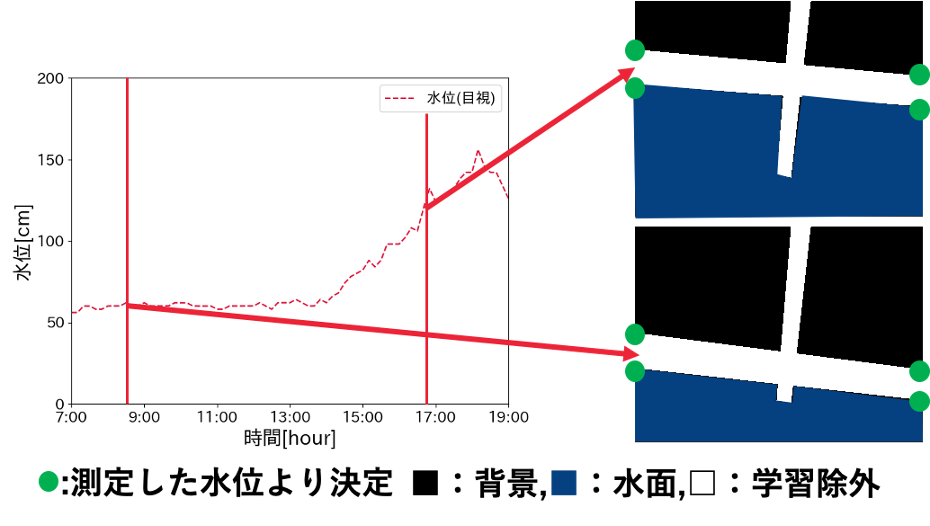
\includegraphics[keepaspectratio,scale=0.45]{./figs/ano2.png}
    \vspace{-5mm}
    \caption{範囲設定の流れ}
    \vspace{-5mm}
    \label{images_range}
\end{figure}

また,水面領域の面積割合から水位へ値を変換する式を作成し,
領域抽出結果画像から水位の推定値への変換を行った.


\section{実験}

\begin{table}[b]
  \centering
  \begin{tabular}{lrr}
     &IoU&F値\\ \hline 
   設定A&92.30& 95.94\\ \hline  
   設定B&88.57&  93.89\\ \hline 
  \end{tabular}
  \vspace{-3mm}
  \caption{IoU(%)とF値(%)}
  \label{pole_AB}
\end{table}

SS手法と先行研究\cite{watanabe}の手法(以後,先行手法)の比較を行う前に,水位計測ポールに対する適切なラベル設定の調査するために,
2種類のアノテーション設定で構築したモデルの領域抽出精度の比較を行った.そして,精度が高い方の設定を先行手法
との比較で使用した.
設定Aは水面と撮影日時に水面ラベル(撮影日時の範囲よりも下に水面がくる場合が無いため),壁面に背景ラベル,水位計測ポールを学習除外領域に設定した.
また,設定Bは水位計測ポール以外は設定Aと統一し,水位計測ポールに水位計測ポールラベルを与えた.

SS手法の精度を評価するため,監視カメラに先行手法とSS手法を適用し,
推定した水位と目視で計測した水位との誤差を比較した.
畳込みニューラルネットワークによるセマンティックセグメンテーションのシステムとして,
DeepLabv3+\cite{deeplabv3+}を用いた.
訓練データとして,2018年7月6日の7:00から19:00の画像データ(8147枚)を用いた.
テストデータとして,同年7月7日同時間帯の画像データ(8086枚)を用いた.

\section{結果と考察}
\subsection{先行研究との比較結果}



設定A,Bの水面クラスのIoU\cite{IoU}とF値\cite{bf}は表\ref{pole_AB}の通りとなった.今回は
水面の領域抽出精度の調査のため,水面クラスに注目して領域抽出精度を評価した. 
両設定で高い抽出精度が確認されたが,設定Aの方がIoUとF値が良い結果になることが確認できた.
よって,先行手法との比較は設定Aを用いて行った.



\begin{figure}[t]
    \begin{minipage}[b]{0.49\linewidth}
      \centering
      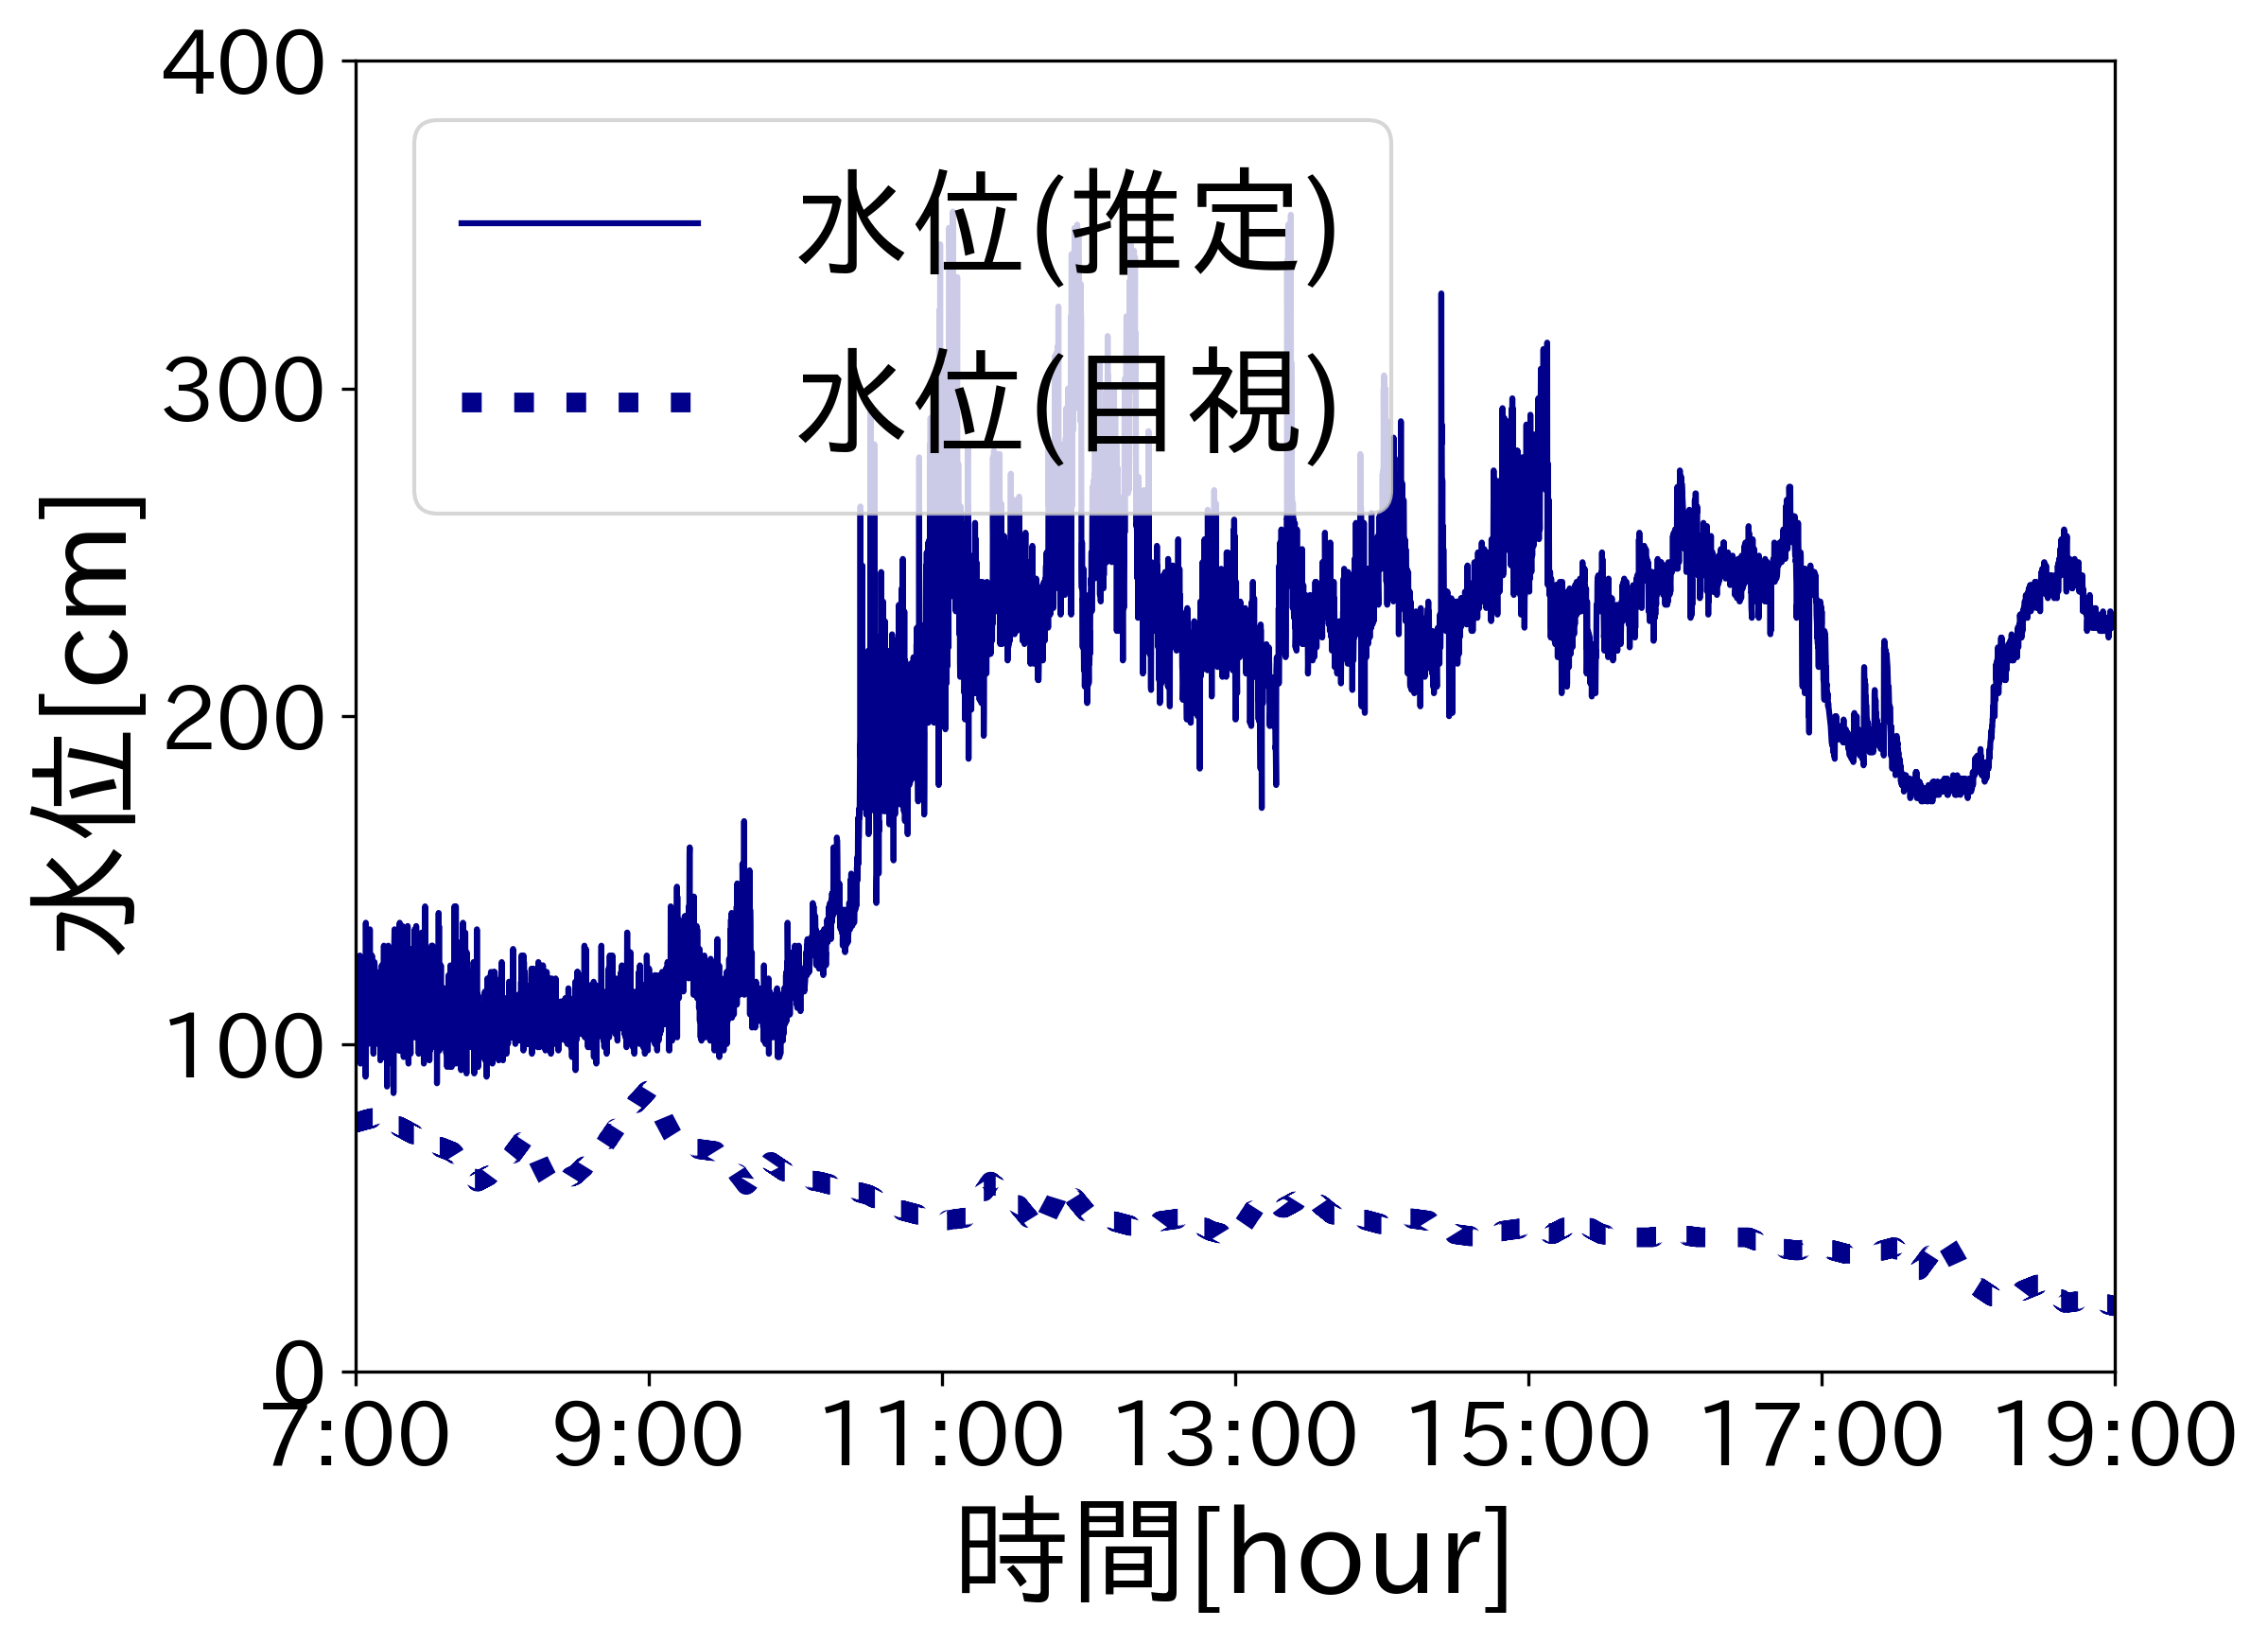
\includegraphics[keepaspectratio,scale=0.2]{graph/A.png}
      \vspace{-5mm}
      \subcaption{先行研究}
    \end{minipage}
    \begin{minipage}[b]{0.49\linewidth}
      \centering
      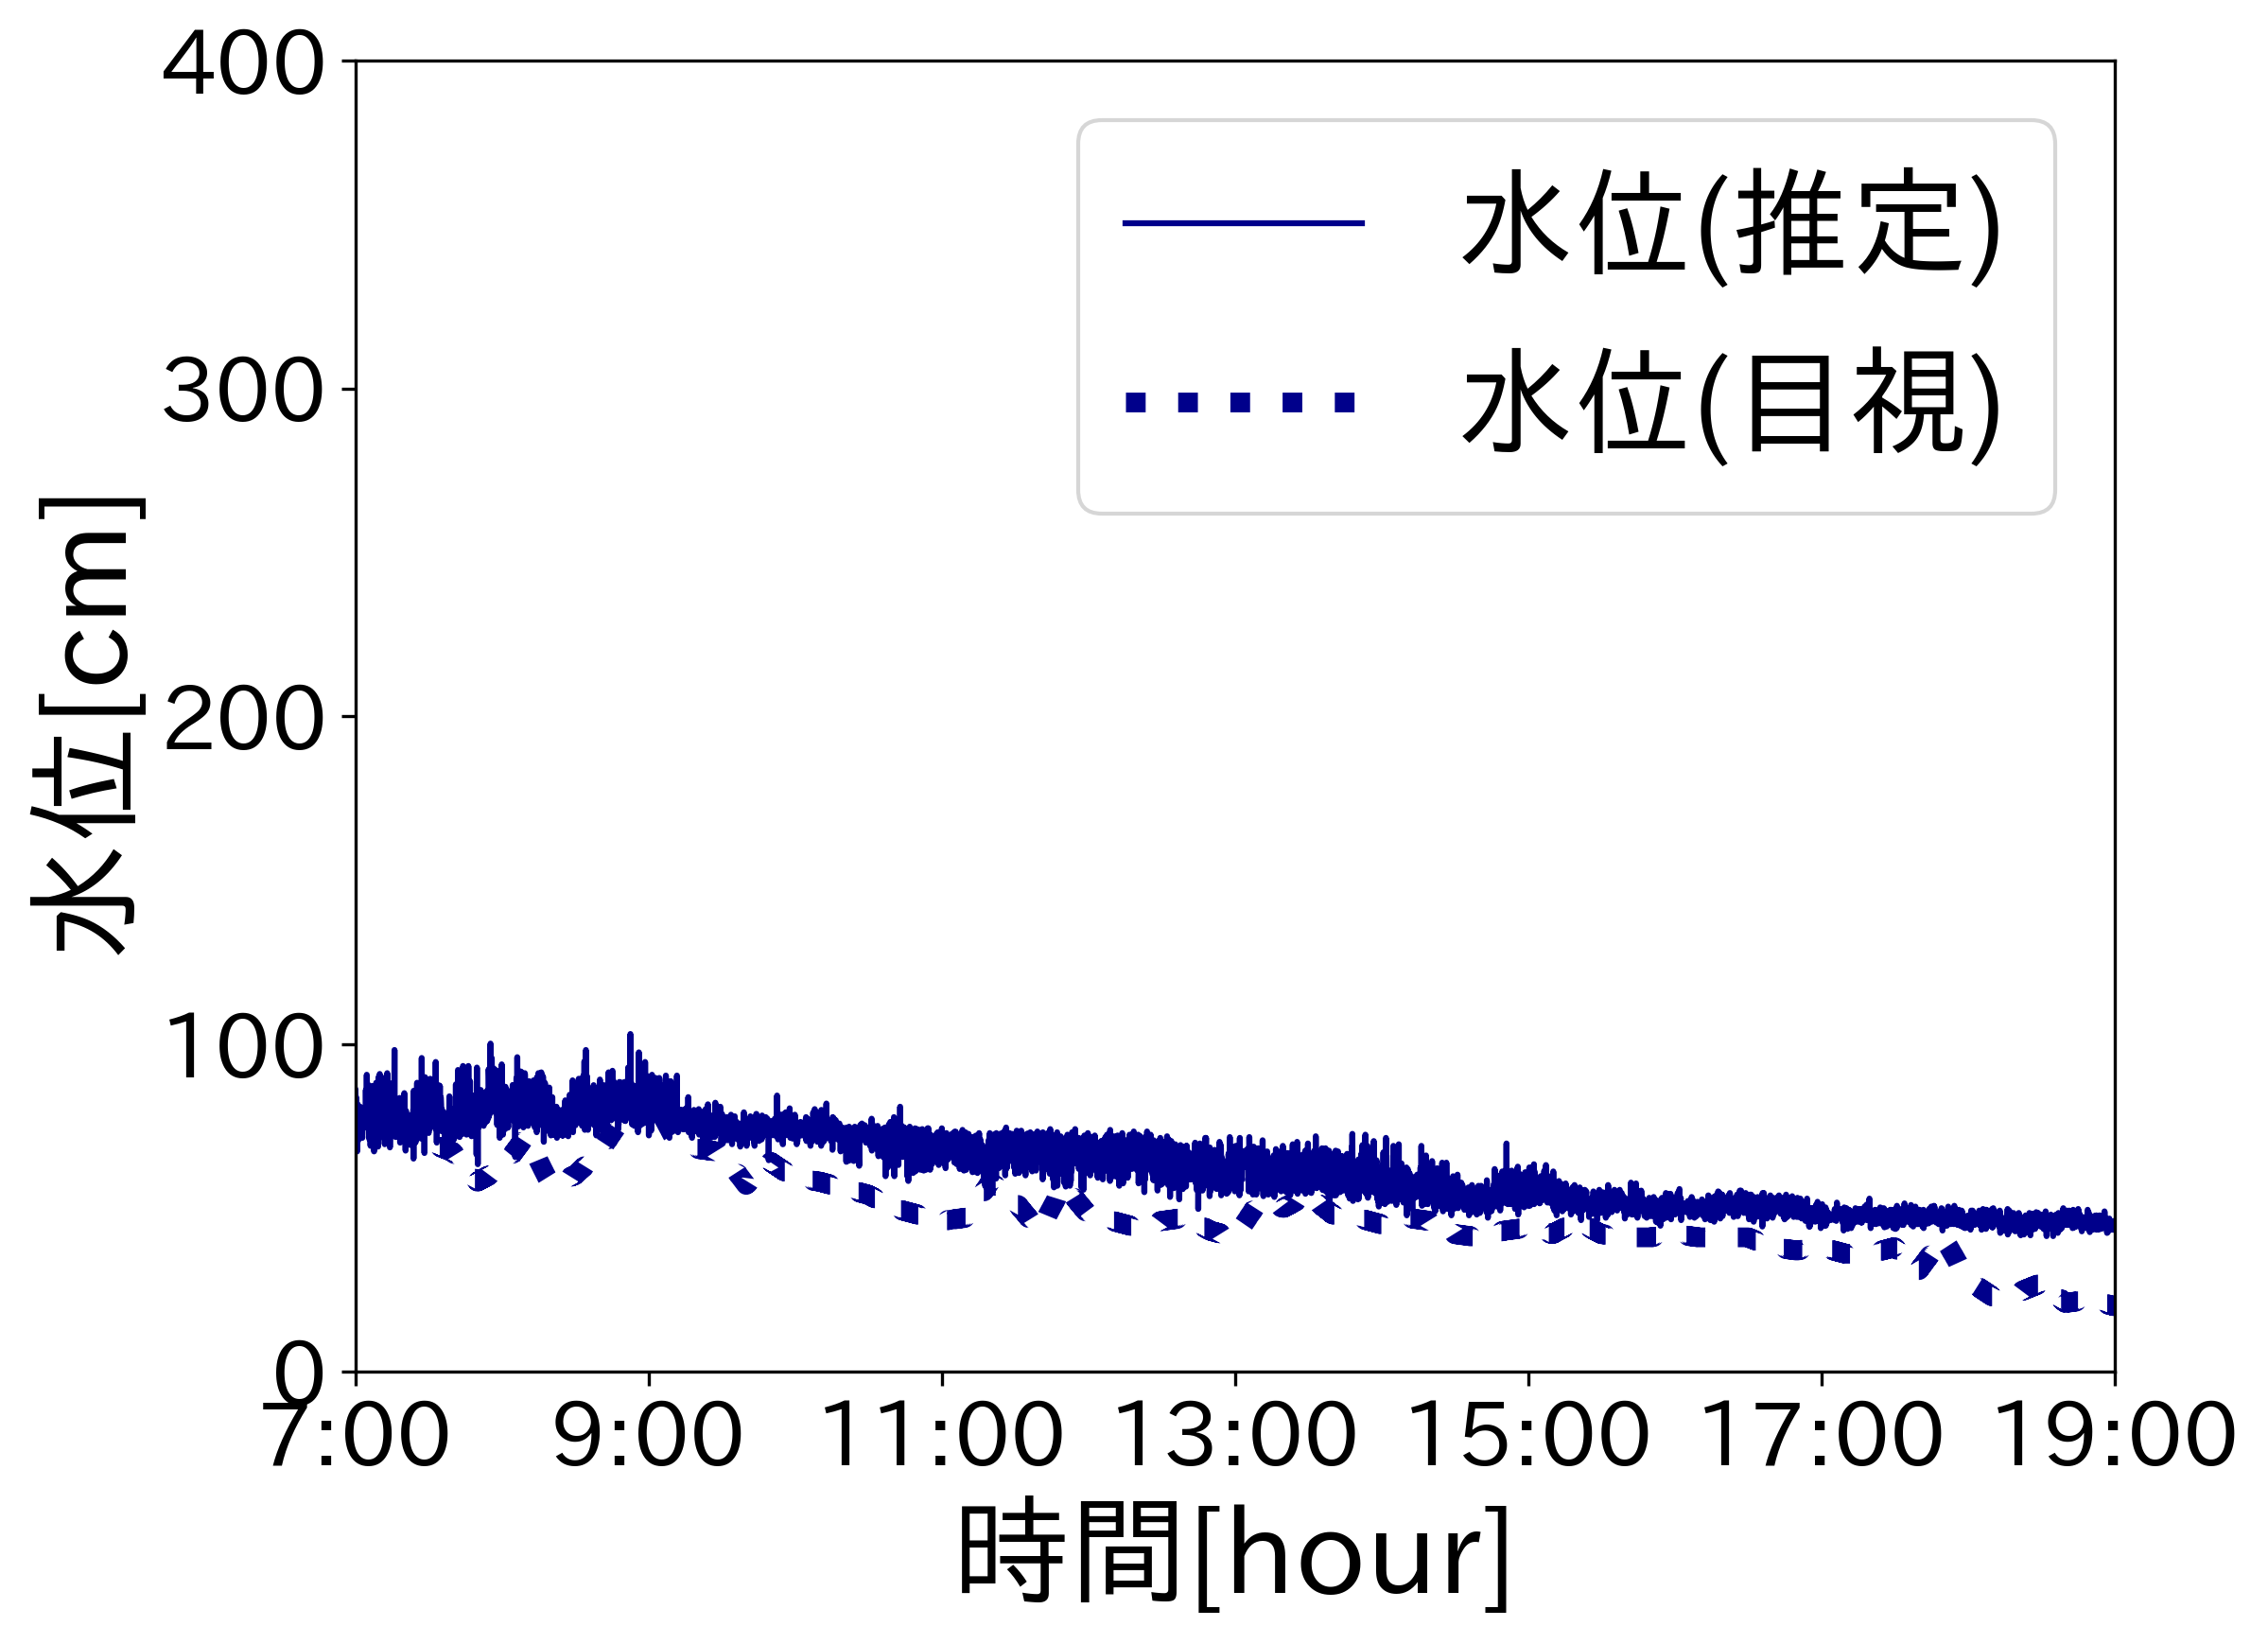
\includegraphics[keepaspectratio,scale=0.2]{graph/SS.png}
      \vspace{-5mm}
      \subcaption{SS手法}
    \end{minipage}
    \vspace{-7mm}
    \caption{2018年7月7日の水位推定結果}
    \vspace{-6mm}
    \label{graph}
\end{figure}


先行手法とSS手法による水位推定の結果を図\ref{graph}に示す.
目視で計測した水位とのRMSE (Root Mean Square Error) は,先行手法で163.44cm,SS手法で15.02cmとなった.
つまり,先行手法と比べSS手法の方がかなり高い精度を達成できた.
また,先行手法には訓練データと異なる日のデータに対して推定精度が低くなるという問題があったが,
SS手法は,訓練データと異なる日のデータに対しても高い推定精度があることが確認できた.

領域抽出精度と水位推定精度の高さから,提案したアノテーション方法とSS手法の有効性を確認できた.

\subsection{交差検証}

\begin{table}[b]
  \centering

  \begin{tabular}{l|rrr}
     &7月5日&7月6日&7月8日 \\ \hline 
   IoU(%)&88.33&91.05&90.36\\ \hline  
   F値(%)&93.76&95.26&94.87\\ \hline  
   RMSE(cm)&17.32& 7.73&8.32\\ \hline  
  \end{tabular}
  \vspace{-3mm}
  \caption{テストデータ日別RMSEと領域抽出精度} 
  \label{kousa}
\end{table}

2018年,7月5,6,7日の3日分の画像データから
SS手法を用いて水位の推定を行った(3日分のデータの内,
2日分のデータを訓練データ,残った1日分のデータを
テストデータとして使用).
作成したモデルで推定した水位と測定値とのRMSEと領域抽出結果のIoU,F値は表\ref{kousa}の通りとなった. 

特に精度が低い抽出結果例を図\ref{images_kousa}の(b),(c),(d)に示す.
精度の高い(a)の結果と(b),(c),(d)を比較して,どのような河川の状況だと抽出精度が低くなるのかを考察する.
(b)の入力画像は(a)と比べて水位が低く,水面が澄んでいる.
この結果から水面が透き通り水面と壁面の境界が曖昧になると,領域抽出精度が下がると考えられる.
7月5日の河川はこの現象が長く続いたため,他の日に比べ抽出精度が少し低くなったと
考えられる.
一方,(c)の入力画像は水面が濁っており,水面と壁面の特徴が近くなっていることが確認できる.そのため,
水面が濁った場合でも領域抽出精度が下がると考えられる.
(d)の入力画像は
水面が波立っており,泡が発生したり,水面と壁面の境界が複雑になっていることが確認できる.
よって,水面の状態が大きく変化することでも,領域抽出精度が下がると考えられる.

また,全ての日のデータに対してIoU,F値が85%以上であることから,作成したモデルは
過学習を起こさずに抽出が行えていることが確認できた.





\begin{figure}[t] 
    \begin{center}
      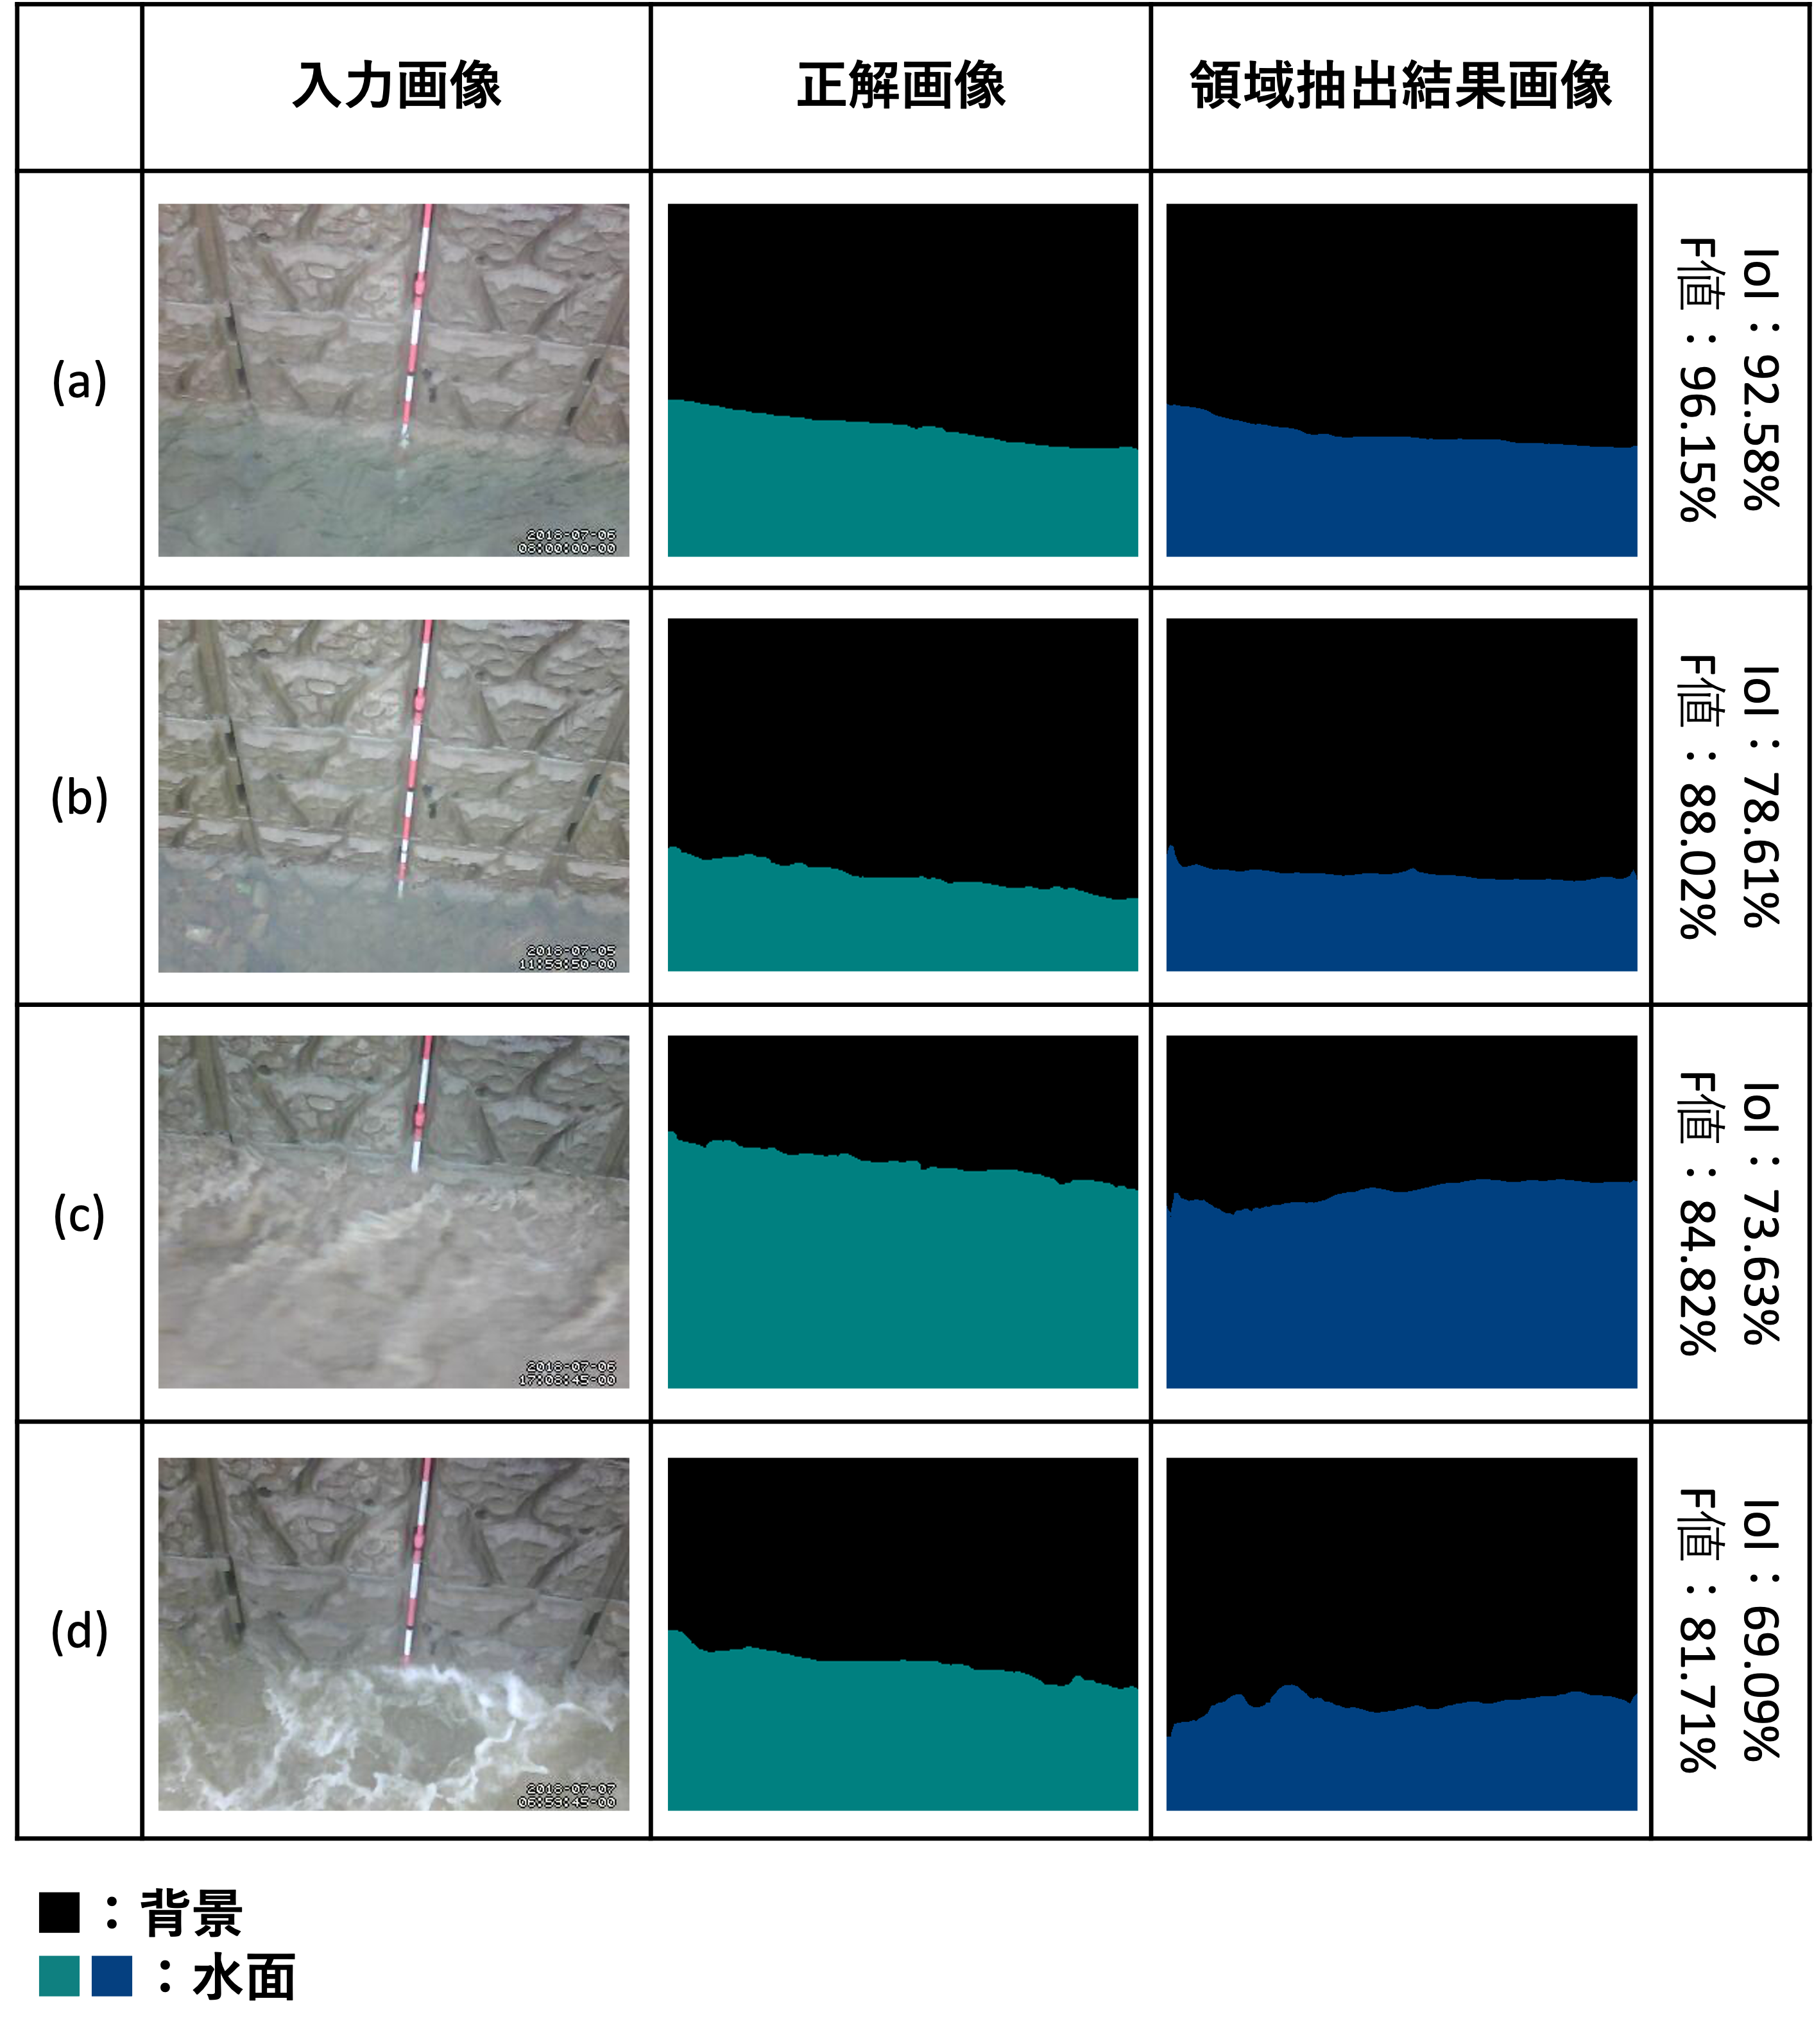
\includegraphics[keepaspectratio,scale=0.355]{./figs/kousa_1.png}
    \end{center}
    \vspace{-8mm}
    \caption{領域抽出結果例}
    \vspace{-6mm}
    \label{images_kousa}
\end{figure}


\section{まとめと今後の課題}
\vspace{-1mm}

本研究では,深層学習を用いたセマンティックセグメン
テーションによって河川の監視カメラ画像から水位を推定することを目的とし,
訓練データとして必要なアノテーション画像を半自動的に作成する方法を提案した.
交差検証を行った結果,提案手法を用いて作成したモデルは全て
のテスト日でIoUとF値が85%以上となった.
しかし,水面の状態によって精度が低くなるといった問題が見受けられた.
また,水位の推定方法としてSS手法を検討した.
SS手法と先行手法を適用して水位を推定し,
目視で測定した水位との誤差を利用して評価を行った.
その結果,SS手法のRMSEが15.02cm,先行手法が163.44cmとなり,
SS手法を用いた場合の誤差の方が小さくなった.
今後の課題としては,夜間といった異なる条件下に対する適用実験やアノテーション画像の自動生成などが
挙げられる.

%参考文献
\begin{thebibliography}{9}

  \bibitem{mlit}
  国土交通省:
  令和4年の土砂災害発生件数は795件,
  砂防NEWS Press Release,2023年3月.
      
  \bibitem{watanabe}
  渡邊 康平:
  土砂災害の前兆現象検知を目的とした画面分割と深層学習を用いた水位変動の推定,
  広島市立大学大学院情報科学研究科システム工学専攻修士論文,
  2023年1月.
      
  \bibitem{seman}
  N,A.Muhadi,A.Mijic,A.F.Abdullah,
  S.K.Bejo,M.R.Mahadi:
  Deep Learning Semantic Segmentation for Water Level Estimation Using Surveillance Camera,
  Applied Sciences,vol.11,issue.20,(2021).
    
  
  \bibitem{deeplabv3+}
  Chen,L.C.,Zhu,Y.,Papandreou,G.,Schroff,F.,Adam,H.:
  Encoder-decoder with atrous separable convolution for semantic image segmentation.
  In Proceedings of the European conference on computer vision (ECCV) (pp. 801-818).(2018).
      
  \bibitem{IoU}
  青島亘佐, 山本拓海,中野聡,中村秀明:
  深層学習によるセグメンテーション手法を用いたコンクリート表面の変状領域の検出.
  AI・データサイエンス論文集,1(J1),481-490.2020年).
      
  \bibitem{bf}
  山根達郎,全邦釘: 
  Deep learning による Semantic Segmentation を用いたコンクリート表面ひび割れの検出.
  構造工学論文集 A,65,130-138.(2019年).
      
\end{thebibliography}
    
\end{document}
